% This is an example of how to create a presentation in PDFLaTeX. 
% Matt Welsh, mdw@cs.berkeley.edu
% See http://www.cs.berkeley.edu/~mdw/proj/texslides for details.

% The basic document style is 'foils' from the FoilTeX package
\documentclass[20pt,landscape]{foils}
% These are my macros for creating slides
\usepackage{mdwslides}

% Basic things that we need are below
\usepackage[english]{babel}
\usepackage{hyperref}
\hypersetup{
  pdfmenubar=true,
  pdftoolbar=true,
  pdfpagemode={None}
}
\usepackage{pause}
\usepackage{graphicx}
\usepackage[utf8]{inputenc}
\inputencoding{utf8}
%%%%%%%%%%%%%%%%%%%%%%%%%%%%%%%%%%%%%%%%%%%%%%%%%%%%%%%%%%%%%%%%%%%%%%%%%%%%

% Set headers
\MyLogo{Ole Aamot}
\rightfooter{\quad\textsf{\thepage}}

\begin{document}
\rm

\slide{}
\LogoOff

\vskip 1.5in
\begin{center}
  {\color{mdwblue}\Large\slingbold GNOME Internet Radio Locator
    
    \vskip 11ex
    Ole Aamot
    \vskip 1ex
           {\small\trebucit ole@src.gnome.org}
           \vskip 1ex
                  {\mdwsmall\tt http://girl.software/}
                  }
\end{center}

\slide{Introduction}
\LogoOn
GIRL, the GNOME Internet Radio Locator program, allows users to easily find and record live radio programs on radio broadcasters on the Internet.

GIRL is developed for the GNOME desktop and requires one audio helper such as GNOME Videos (\url{https://wiki.gnome.org/Apps/Videos}) to be installed for playback and streamripper (\url{http://streamripper.sourceforge.net/}) to be installed for recording live radio streams of supported radio stations. 

GIRL, a recursive acronym for GNOME Internet Radio Locator,
following the tradition of naming projects in Free Software
culture.

GIRL is not officially a part of GNU or GNOME, but using the
*.gnome.org infrastructure on \url{http://git.gnome.org/girl}
and \url{https://download.gnome.org/sources/girl/}

\slide{Why did I write GNOME Internet Radio Locator (GIRL)?}

\begin{list1}
\item 
  \begin{list2}
  \item I support
    \begin{list3}
    \item Freedom
    \item Free Speech
    \item Free Software
    \end{list3}
  \item I want to give something back to the Free Software community    
  \item Internet Radio is a free Internet resource
  \item Many Universities run non-profit Internet radio stations
  \end{list2}
\end{list1}

\slide{History of GNOME Internet Radio Locator}

\begin{list1}
\item 2002
  \begin{list2}
  \item Test client for streaming Radio NOVA / radiOrakel / Radio Tellus live
  \item GIRL 0.1.0 released at 01lab at Norwegian Computing Center in 2002.
  \item GIRL 0.1.0 just sat on my backups/machines/harddrives 2002 - 2014.
  \end{list2}
\item 2014
  \begin{list2}
  \item Visit to SIPB at MIT in June 2014 inspired me to release GIRL 0.2.0.
  \end{list2}
\item 2015
  \begin{list2}
    \item GIRL 1.0.0 released on January 3rd, 2015 with 42 Internet radio stations
    \item GIRL 1.0.0 named ``Fenchurch'' as tribute to Terry Pratchett's Discworld
    \item GIRL 2.0.0 released on March 29th, 2015
    \item GIRL 3.0.0 released on April 25th, 2015
    \item GIRL 4.0.0 released on May 3rd, 2015
    \item GIRL 5.0.0 released on May 8th, 2015 with 73 Internet Radio stations
  \end{list2}
\end{list1}

\slide{What is the definition of Free Software?}

From FSF's home page (\url{https://www.gnu.org/philosophy/free-sw.html}):

\begin{list1}
\item Free Software is a good idea because you have
  \begin{list2}
    \item The freedom to run the program as you wish, for any purpose (freedom 0).
    \item The freedom to study how the program works, and change it so it does your computing as you wish (freedom 1). Access to the source code is a precondition for this.
    \item The freedom to redistribute copies so you can help your neighbor (freedom 2).
    \item The freedom to distribute copies of your modified versions to others (freedom 3). By doing this you can give the whole community a chance to benefit from your changes. Access to the source code is a precondition for this.
  \end{list2}
\end{list1}

\slide{Existing Music Services}

\begin{list1}
\item Apple iTunes, Google Music and Spotify
  \begin{list2}
  \item Require non-free client software
  \item DRM (Digital Restrictions Management)
  \item Impose EULAs that restrict more than copyright
  \item Track what the user listens to
  \end{list2}
\end{list1}

One redeeming feature of some of them:

\begin{list2}
\item You can't access them from GNU/Linux at all.  If you're a GNU/Linux user, this protects you from the temptation to use them.
\end{list2}

\slide{Why did I write GIRL?}

The last public talk I gave, was a talk on Music Recording, Production and Distribution with Free Software at UKUUG Linux 2005 at University of Wales, Swansea, in 2005. The talk is available from \url{http://home.nuug.no/~ole/UKUUG2005.pdf}

10 years is a long time, a lot of stuff has happened in these 10 years.

\begin{list1}
\item Free Radio
\item Free Speech
\item Free Software
\end{list1}

\slide{Features in GNOME Internet Radio Locator version 5.0.0} 

\begin{list1}
\item 73 non-profit and independent radio stations are supported.
\item 14 language translations (see girl/AUTHORS and girl/THANKS).
\item Radio station search by physical location, but just city names.
\item Optional recording feature (if ``streamripper'' is available)
\item Support for Personal Radio Stations (``\$HOME/.girl/girl.xml'').
\item Play supported radio codecs with GNOME Videos
\end{list1}

\slide{Supported Internet Radio Stations}

The following 73 radio stations are supported in GIRL 5.0.0:

\begin{list1}
\item
  \begin{list2}
  \item 2NURFM (Newcastle, Australia)
  \item 95bFM (Auckland, New Zealand)
  \item Arizona State University (Phoenix, AZ)
  \item BBC World Service (London, United Kingdom)
  \item Burst Radio (Brighton, United Kingdom)
  \item CFRC (Kingston, Canada)
  \item CHUO (Ottawa, Canada)
  \item CJSW (Calgary, Canada)
  \item COOG (Houston, TX)
  \item Cam FM (Cambridge, United Kingdom)
  \item Caper Radio (Sydney, Nova Scotia, Canada)
  \item Coimbra University Radio (Coimbra, Portugal)
  \item EPER (Budapest, Hungary)
  \item Fuse FM (Manchester, United Kingdom)
  \item Imperial College Radio (London, United Kingdom)
  \item KALX (Berkeley, CA)
  \item KCSN (Los Angeles, CA)
  \item KDUP (Portland, OR)
  \item KEXP (Seattle, WA)
  \item KSUB (Seattle, WA)
  \item KTRU (Houston, TX)
  \item KTUH (Honolulu, Hawaii)
  \item KVRX (Austin, TX)
  \item KXSC (Los Angeles, CA)
  \item KZSU (San Francisco, CA)
  \item King's College London Radio (London, United Kingdom)
  \item Leeds University Student Radio FM (Leeds, United Kingdom)
  \item NRK P1 (Oslo, Norway)
  \item NRK P2 (Oslo, Norway)
  \item NRK P3 (Oslo, Norway)
  \item NRK Radio Alltid Nyheter (Oslo, Norway)
  \item NRK Ur{\o}rt (Oslo, Norway)
  \item Oxford Student Radio (Oxford, United Kingdom)
  \item Pulse LSE (London, United Kingdom)
  \item Radio AF (Lund, Sweden)
  \item Radio Adelaide (Adelaide, Australia)
  \item Radio Campus Bruxelles (Bruxelles, Belgium)
  \item Radio Campus Paris (Paris, France)
  \item Radio Eco (Pisa, Italy)
  \item Radio NOVA (Oslo, Norway)
  \item Radio NRJ Bern (Bern, Switzerland)
  \item Radio R (Brno, Czech Republic)
  \item Radio Radius (Zürich, Switzerland)
  \item Radio UNAM (México City, México)
  \item RÚV (Reykjavik, Iceland)
  \item SoundFM (Waterloo, Canada)
  \item Stockholm College Radio (Stockholm, Sweden)
  \item UCT Radio (Cape Town, South Africa)
  \item University Radio Nottingham (Nottingham, United Kingdom)
  \item University Radio York (York, United Kingdom)
  \item WAMU (Washington, DC)
  \item WCSB (Cleveland, OH)
  \item WHPK (Chicago, IL)
  \item WHRB (Boston, MA)
  \item WKCR (New York City, NY)
  \item WMBR (Boston, MA) 
  \item WNYO (Oswego, NY)
  \item WPTS (Pittsburgh, PA)
  \item WRVU (Nashville, TN)
  \item WTBU (Boston, MA)
  \item WUMR (Memphis, TN)
  \item WUSB (Long Island, NY)
  \item WVAU (Washington, DC)
  \item WVUA-FM (Tuscaloosa, AL)
  \item WWNO (New Orleans, LA)
  \item WXOU (Rochester, MI)
  \item WXYC (Chapel Hill, NC)
  \item radiOrakel (Oslo, Norway)
  \end{list2}
\end{list1}

See \url{http://girl.software/girl.xml} for the current list of supported
radio stations in GNOME Internet Radio Locator.

\slide{Supported Radio Codecs}

The radio stations stream live audio with several different audio codecs supported by the GNOME Videos program, see \url{https://wiki.gnome.org/Apps/Videos}

The audio codecs in usage among the supported 76 radio stations are:

\begin{list1}
  \item
    \begin{list2}
    \item ``AAC, v4 LC''
    \item ``MPEG 1 Audio, Layer 3 (MP3)''
    \item ``MPEG-2 AAC (AAC+)''
    \item ``MPEG-2 AAC''
    \item ``MPEG-4 AAC''
    \item ``Ogg Vorbis''
    \end{list2}
\end{list1}

\slide{GIRL Data Type Definition (DTD)}

\begin{list1}
\item GIRL 0.1 DTD began at Norwegian Computing Centre in 2002.
\item Short description of each radio station (<station ...>).
\item Short description of each radio station stream (<stream ...>).
\item GIRL 5.0 DTD is available from \url{http://girl.software/girl-5.0.dtd}
\item GIRL 5.0 XML data renders as HTML using XSLT in at least Firefox 36.0 at \url{http://girl.software/girl.xml}
\end{list1}


\slide{Current GIRL 5.0 DTD}

\begin{tiny}
\begin{verbatim}
<!ATTLIST frequency uri CDATA #REQUIRED >
<!ELEMENT description ( #PCDATA ) >
<!ATTLIST description lang CDATA #REQUIRED >
<!ELEMENT frequency ( #PCDATA ) >
<!ELEMENT location ( lat | lon )* >
<!ELEMENT girl ( station+ ) >
<!ATTLIST girl version NMTOKEN #REQUIRED >
<!ELEMENT station ( frequency | location | description | stream)* >
<!ATTLIST station band CDATA #REQUIRED >
<!ATTLIST station icon CDATA #REQUIRED >
<!ATTLIST station id NMTOKEN #REQUIRED >
<!ATTLIST station lang CDATA #REQUIRED >
<!ATTLIST station name CDATA #REQUIRED >
<!ATTLIST station rank CDATA #REQUIRED >
<!ATTLIST station type CDATA #REQUIRED >
<!ELEMENT stream EMPTY >
<!ATTLIST stream bitrate NMTOKEN #REQUIRED >
<!ATTLIST stream channels NMTOKEN #IMPLIED >
<!ATTLIST stream codec CDATA #REQUIRED >
<!ATTLIST stream mime CDATA #REQUIRED >
<!ATTLIST stream samplerate NMTOKEN #REQUIRED >
<!ATTLIST stream uri CDATA #REQUIRED >
\end{verbatim}
\end{tiny}

\slide{Example of GIRL 5.0 XML data}

\begin{tiny}
\begin{verbatim}
<?xml version="1.0" encoding="UTF-8"?>
<?xml-stylesheet type="text/xsl" href="http://girl.software/girl.xsl" ?>
<!DOCTYPE girl SYSTEM "girl-5.0.dtd">
<girl version="5.0">
  ...
  <station band="88.1FM"
           id="wmbr"
           lang="en"
           name="WMBR"
           rank="1.0"
           type="edu">
    <frequency>88.1 FM in Cambridge, MA</frequency>
    <location>Boston, MA</location>
    <description lang="en">WMBR is the MIT campus radio station.
    We broadcast on 88.1 FM between 20 and 24 hours per day, 365 days a year.
    We transmit at 720 watts, effective radiated power from the top of the
    Eastgate Building in Kendall Square in Cambridge, Massachusetts.
    Our programming includes a wide range of music shows, public affairs
    programs and eclectic audio entertainment.</description>
    <stream mime="audio/mpeg"
            uri="http://wmbr.org/WMBR_live_128.m3u"
            codec="MPEG 1 Audio, Layer 3 (MP3)"
            samplerate="44100 Hz"
            channels="Stereo"
            bitrate="128 kbps" />
    <uri>http://wmbr.org/</uri>
  </station>
  ...
</girl>
\end{verbatim}
\end{tiny}

\slide{Screenshot}

\begin{center}

  \colorbox{white}{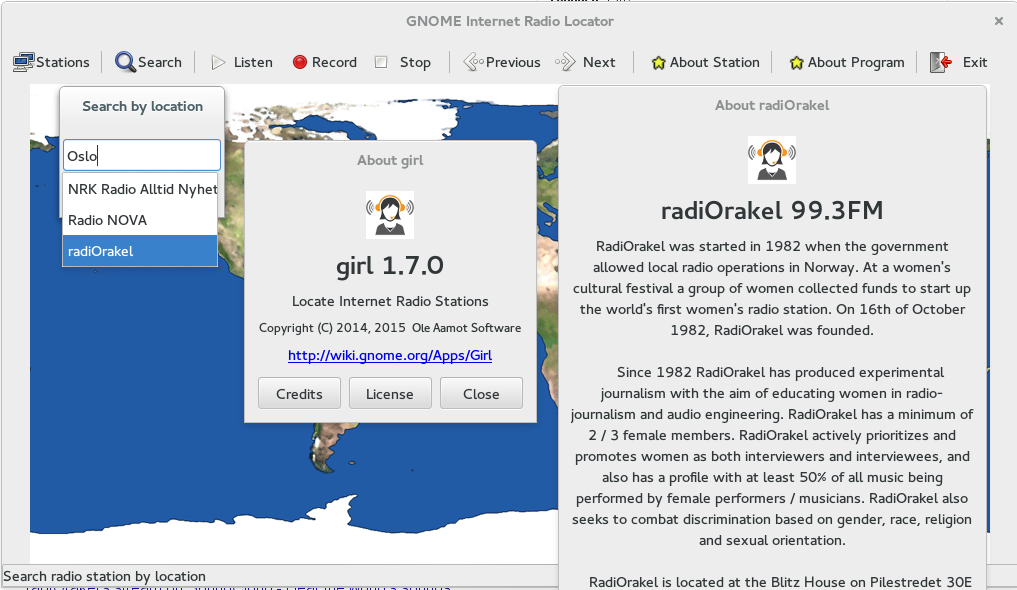
\includegraphics[width=0.6\hsize]{../data/screenshot.png}}

  {\blueem Screenshot of GNOME Internet Radio Locator 5.0.0}

\end{center}

\slide{Legal stuff}

\begin{list1}
  \item Internet Radio stations in the U.S. need a broadcast license permit from the F.C.C.
    \begin{list2}
    \item Read girl/BROADCAST for some details on radio and music licensing
    \item \url{http://en.wikipedia.org/wiki/Broadcast_license}
    \item \url{https://www.dnalounge.com/backstage/webcasting.html}
    \end{list2}
  \item Personal Radio Stations can be set up using Icecast streaming server
    \begin{list2}
    \item Download Icecast from \url{http://www.icecast.org/} and add your station in \$HOME/.girl/girl.xml
    \end{list2}
  \item Only Internet radio stations with broadcast permit are included in GIRL
\end{list1}

\slide{Internet Radio Fairness Act}

\begin{list1}
\item Many Internet radio stations can't afford to pay royalty fee collection agencies
  \begin{list2}
  \item The American Society of Composers, Authors and Publishers (ASCAP)
  \item Broadcast Music, Inc. (BMI)
    \item Society of European Stage Authors and Composers (SESAC)
  \end{list2}
  \item New bill in support of Internet Radio introduced in U.S. Congress 2002:
  \begin{list2}
  \item \url{https://www.eff.org/Internet-Radio-Fairness-Act-Explanation}
  \item \url{http://en.wikipedia.org/wiki/Internet_Radio_Equality_Act}
  \end{list2}
\item EFF had a 2012 campaign in support of the Internet Radio Fairness Act
  \begin{list2}
  \item \url{https://www.eff.org/Internet-Radio-Fairness-Act-Explanation}
  \end{list2}
\item A recommended letter to U.S. congress representatives is included in GIRL
  \begin{list2}
  \item See girl/LETTER and \url{http://girl.software/LETTER.html}
  \end{list2}
\item The IRFA bill may be reintroduced in U.S. Congress in 2016, but who knows?
\end{list1}

\slide{Email from Dr. Richard M. Stallman of FSF}

\begin{list1}
\item
  \begin{tiny}
\begin{verbatim}
    From: Richard Stallman <rms@gnu.org>
    Subject: Re: Internet Radio Fairness Act? (Re: It's your birthday)
    Date: Mon, 23 Mar 2015 22:43:25 -0400
    To: oka@oka.no

    [[[ To any NSA and FBI agents reading my email: please consider    ]]]
    [[[ whether defending the US Constitution against all enemies,     ]]]
    [[[ foreign or domestic, requires you to follow Snowden's example. ]]]

      > Regarding updating the LETTER included in GNOME Internet Radio Locator,
      > I don't know what to write/who to contact to promote Internet Radio
      > Fairness Act again in U.S. politics, except you.

    Ask people to contact their congressional representatives.

    Can you write a message to the public about this?

    -- 
    Dr Richard Stallman
    President, Free Software Foundation
    51 Franklin St
    Boston MA 02110
    USA
    www.fsf.org  www.gnu.org
    Skype: No way! See stallman.org/skype.html.
\end{verbatim}
  \end{tiny}
\end{list1}  

\slide{Questions?}

\begin{list1}
\item GNOME Internet Radio Locator 5.0.0 is available here and now.
  \begin{list2}
  \item \url{http://download.gnome.org/sources/girl/5.0/girl-5.0.0.tar.xz}
  \end{list2}
\item Debian 8.0 'jessie' packages
  \begin{list2}
  \item \url{http://girl.software/girl_5.0.0-1_i386.deb}
  \end{list2}
\item Fedora 21 RPMS
  \begin{list2}
  \item \url{http://girl.software/girl-5.0.0-1.fc21.x86_64.rpm}
  \end{list2}
\item Mailing List    
  \begin{list2}
  \item \url{http://mail.gnome.org/mailman/listinfo/girl-list/}
  \end{list2}
\item Source repository
  \begin{list2}
    \item \url{git://git.gnome.org/girl}
    \item \url{https://git.gnome.org/browse/girl}
    \item \url{ssh://$USERNAME@git.gnome.org/git/girl}
  \end{list2}
\end{list1}

\end{document}
